\chapter{Fluid Simulation}\label{chapter:fluid-simulation}
Simulating convincing fluid dynamics is a continuing challenge of computer
graphics, especially when considering real-time applications. There are multiple
established ways to simulate fluids, the most widespread being Eulerian (i.e.
grid-based) and Lagrangian (i.e. particle-based) methods. Here, we restrict
ourselves to discussing Eulerian methods, and also introduce the Laplacian
Eigenfunction method, introduced by \cite{dewitt}.

The dynamics of fluids are governed by the Navier-Stokes Equations:
\begin{equation}\label{eq:NSE}
    \pdv{\vb{u}}{t} + (\vb{u}\cdot\grad)\vb{u}
    = -\frac{1}{\rho}\grad{p} + \nu\grad^2\vb{u} + \vb{f},
\end{equation}

where $\vb{u}$ is the velocity of the fluid, $\rho$ is the density, $p$ is the
scalar pressure field, $\nu$ is the viscosity constant, and $\vb{f}$ denotes
external forces. For incompressible fluids, the divergence-freeness also has to
hold, i.e. $\div{\vb{u}} = 0$

Even though equation~\eqref{eq:NSE} already describes the evolution of the fluid
as a \acf{PDE}, it is too complex for simply stepping it forward in time with
Euler steps. Instead, a technique called \textit{operator splitting} is applied
for numerical simulations, where each term is treated individually, and their
effect is combined to fully approximate the original equation. We give
a short overview of each term to get a general understanding of fluid
simulation, first treating the problem in an Eulerian way (i.e.  sampling
$\vb{u}$ on a grid), building up our way towards the Laplacian Eigenfunction
method discussed in section~\ref{section:laplacian-eigenfluids}.  For a more
complete overview of established fluid simulation techniques, see
\cite{FluidNotes} and \cite{BridsonFluid}.

Equation~\eqref{eq:NSE} is usually split by separating out the advection part,
the external force part, and the pressure/incompressibility part. When viscosity
is important, that can also be separated. This means, we work out methods for
solving these simpler equations:
\begin{align*}
    \dv{q}{t} &= 0              \qq{(advection)}\\
    \pdv{\vb{u}}{t} &= \vb{f}   \qq{(external forces)}\\
    \pdv{\vb{u}}{t} + \frac{1}{\rho}\grad p &= 0 \\
    \qq{such that}\div{\vb{u}} &= 0.
                                \qq{(pressure, enforcing incompressibility)}
\end{align*}

A generic quantity $q$ is used in the advection equation, because as we also
show later on in our experiments, we may be interested in advecting other field
quantities than just the velocity $\vb{u}$. For the advection part, the
$\text{Advect}(\vb{u}, \Delta t, q)$ algorithm is introduced: it advects
quantity $q$ through the velocity field $\vb{u}$ for a time interval $\Delta t$. 

For the external forces, any traditional numerical integration approach, such as
a simple Euler step can be used: $\vb{u}^{t+1} = \vb{u}^t + \Delta t \vb{f}$.
(See section~\ref{section:numerical-integration}.)

For calculating the pressure, an algorithm $\text{Project}(\Delta t, \vb{u})$
calculates and applies just the right amount of pressure to the velocity field
to make it divergence-free, and also enforce any solid wall boundary
conditions. The term "project" comes from the fact that the algorithm
essentially projects $\vb{u}$ to the closest divergence-free velocity field, and
interpreting the difference between these two fields as a pressure resulting
from "particles" being too close together. We do not go into the details of a
pressure solve here, as our velocity field $\vb{u}$ from the Laplacian
Eigenfunction method (section~\ref{section:laplacian-eigenfluids}) will already
be divergence-free by construction. 

Note that the order in which these algorithms are being applied matters a lot,
as the advection must be done on a divergence-free field. Putting all of these
together, a basic fluid simulation algorithm can be written as:

\begin{algorithmic}
    \State $\vb{u}^0 \gets \text{an initial divergence-free velocity field}$
    \For{$t = 0, 1, 2 \dots $}
        \State $\Delta t 
            \gets \text{a suitable timestep to go from $t_n$ to $t_{n+1}$}$
        \State $\widetilde{\vb{u}} 
            \gets \text{Advect}(\vb{u}^n,\Delta t, \vb{u}^n)$
        \State $\widetilde{\vb{u}} 
            \gets \widetilde{\vb{u}}^n + \Delta t \vb{f}$
        \State $\vb{u}^{n+1}
            \gets \text{Project}(\vb{u}^n,\Delta t, \vb{u}^n)$
            \EndFor \Comment{$[\vb{u}^0, \dots, \vb{u}^t]$ is the simulated
            fluid flow for $t$ timesteps.}
\end{algorithmic}

\subsection*{Advect}
Before moving on, we briefly discuss the Advect algorithm on grids. As already
shown in section~\ref{eq:material-derivative}, we can write out the advection 
$\dv{q}{t}$ in 3D as
$$\pdv{\vb{u}}{t}\dv{t}{t} 
                    + \pdv{\vb{u}}{x}\dv{x}{t} 
                    + \pdv{\vb{u}}{y}\dv{y}{t} 
                    + \pdv{\vb{u}}{z}\dv{z}{t}$$

A simple and physically-motivated advection approach, called the semi-Lagrangian
method was introduced by \cite{StableFluids}.  Advection in a Lagrangian frame
is trivial: moving particles through a velocity field $\vb{u}$ automatically
solves $\dv{q}{t} = 0$. (Which is something we will fundamentally base our
experiments on in chapter~\ref{chapter:controlling-laplacian-eigenfluids}.) 

To find a new value $q$ at some point $\vb{x}$ in space, the semi-Lagrangian
method conceptually finds the partically, that ended up there from the previous
timestep. As we know that the ``particle'' ended up at $\vb{x}$ from the previous
time step, we can trace it backwards through the velocity field to find where it
came from, grabbing the old value of $q$ at that previous point. When simulating
on a grid, but the start point was not on the grid, then interpolation is
applied.

For tracing a particle at position $\vb{x}$ \textit{backwards} in time by
$\Delta t$ through a velocity field $\vb{u}$, we can utilize integration schemes
introduced in section~\ref{section:numerical-integration}.  The simplest way is
an Euler step: 

$$\vb{x}_{\text{old}} = \vb{x} - \Delta \vb{u}(\vb{x}).$$

In practice, it is advised to apply at least a midpoint method: 
\begin{align*}
    \tilde{\vb{x}} &= \vb{x} - \frac{1}{2}\Delta t \vb{u}(\vb{x})\\
    \vb{x}_{\text{old}} &= \vb{x} - \Delta t \vb{u}(\tilde{\vb{x}}).
\end{align*}

Once we calculated $\vb{x}_{\text{old}}$, we can now simply grab the value of
$q$ from the previous timestep from there, and assign it to our new position in
the current timestep, i.e. $q^{t}(\vb{x}) = q^{t-1}(\vb{x}_{\text{old}})$.

For our smoke simulation examples in
\ref{chapter:controlling-laplacian-eigenfluids} , we are using a MacCormak
advection scheme (\cite{maccormack}) that uses a forward as well as a backward
lookup to estimate and correct the error of the semi-Langrangian advection.

\section{The Laplacian Eigenfunction Method}
\label{section:laplacian-eigenfluids}
\cite{dewitt} introduced the method of using Laplacian eigenfunctions for fluid
simulation. \cite{scalable-eigenfluids} addressed scalability and generalization
issues, and referred to the technique as \textit{eigenfluids}, which we also
adhere to.

The main idea is to express the velocity field $\vb{u}(\vb{x})$ via the linear
combination of $N$ global functions:

\begin{equation}\label{eq:u-lin-comb}
\vb{u}(\vb{x})=\sum_i^N w_i \Phi_i(\vb{x}),
\end{equation}

where the elements of $\vb{w} = [w_0, \dots, w_N]$ are called \textit{basis
coefficients}, and ${\Phi_i}$ are \textit{basis functions}.

As our basis functions, we choose eigenfunctions of the vector Laplacian
operator $\Delta = \grad^2 = \text{grad}(\text{div}) - \text{curl}^2$ (see
section~\ref{section:vector-laplacian}), which further simplifies to $\grad^2
= -\text{curl}^2$ for divergence-free fields.


Besides being eigenfunctions of the vector Laplacian operator, if we further
require our basis fields $\Phi_{\vb{k}}$ to be divergence-free, and to satisfy
a free-slip boundary condition, our basis functions are fully characterized by
\begin{align*}
\nabla^2 \Phi_{\textbf{k}} &= \lambda_{\textbf{k}}\Phi_{\textbf{k}} \\
\nabla \cdot \Phi_{\textbf{k}} &= 0 \\
\Phi_{\textbf{k}} \cdot \textbf{n} &= 0 \text{ at } \partial D,
\end{align*}
where $\textbf{n}$ is the normal vector at boundary $\partial D$.

Closed-form expressions of $\Phi_{\vb{k}}$ exist on the two dimensional $D \in
[0, \pi] \times [0, \pi]$ square domain (\cite{chengfield}). Notating the two
scalar components in the $x$ and $y$ directions $\Phi_{\vb{k}} =(\Phi_{\vb{k},
x}, \Phi_{\vb{k},y})$, we can write them as
\begin{align*}\label{eq:explicit-u}\numberthis
    \Phi_{\vb{k},x}(x, y) &= \eta_{\vb{k}}
    \big( k_2 \sin(k_1 x) \cos(k_2 y) \big) \\
    \Phi_{\vb{k},y}(x, y) &= -\eta_{\vb{k}}
    \big( -k_1 \cos(k_1 x) \sin(k_2 y) \big),
\end{align*}

where $\vb{k} = (k_1, k_2) \in \mathbb{Z}^2$ is the \textit{vector wave number},
$\lambda_{\vb{k}} = -(k_1^2 + k_2^2)$ is the \textit{eigenvalue}, and
$\eta_{\vb{k}} = \frac{1}{-\lambda_{\vb{k}}} = \frac{1}{k_1^2 + k_2^2}$ is
a normalization parameter.  \cite{scalable-eigenfluids} use
$\frac{1}{\sqrt{-\lambda}} = \frac{1}{\sqrt{k_1^2 + k_2^2}}$ for normalization,
but we keep the non-root version, as we did not observe any noticeable
difference between the two during implementation.

As an example, $\Phi_{(4,3)}(x,y)$ is visualized in figure~\ref{fig:phi-example}.
In appendix~\ref{appendix:first_16}, we also plot the first $16$ basis fields.

This a good time to mention that higher wave lengths corresponding to smaller
scales of vorticity has a very literal meaning in our simulation. As we choose
to truncate the spectrum of ${\Phi_k}$ at some number $N$, the error we incur is
well defined: we lose the ability to simulate vortices smaller than a given
scale. Also, as we will see later on, this correspondence to spatial scales of
vorticity lets us control the viscosity (i.e. energy decay) in relation to the
scales of vortices by modifying the base coefficients. By setting the magnitude
of each basis coefficient to decay with a time constant equal to the eigenvalue,
we get the physically correct behavior that small vortices dissipate faster than
large vortices.

\begin{figure}
  \centering
  \begin{subfigure}[t]{0.48\textwidth}
    \centering
    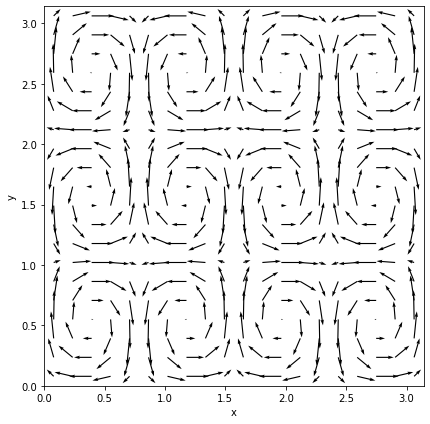
\includegraphics[height=\textwidth]{figures/eigenfluids/k_4_3_vel.png}
    \caption{Velocity field $\Phi_{(4,3)}$.}
  \end{subfigure}
  \begin{subfigure}[t]{0.48\textwidth}
    \centering
    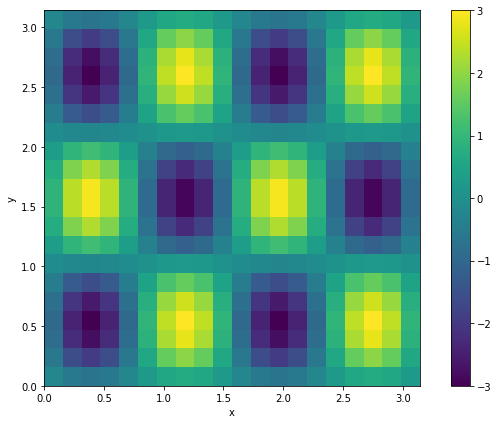
\includegraphics[height=\textwidth]{figures/eigenfluids/k_4_3_curl_bar.png}
    \caption{Curl field $\curl{\Phi_{(4,3)}} = \phi_{(4,3)}$.}
  \end{subfigure}\par\medskip
  \caption{Visualizing $\Phi_{(4,3)}$ sampled on a $20 \times 20$ grid in
  our simulation domain $D = [0,\pi] \times [0,\pi]$.}
  \label{fig:phi-example}
\end{figure}

\subsection*{Vorticity Basis Fields}
For the simulation technique, we further require the vorticity field
$\boldsymbol\omega = \curl{\vb{u}}$ and a set of vorticity basis functions $\phi
= \curl{\Phi}$.  Taking the curl (as introduced in section~\ref{section:curl})
of the velocity basis fields $\Phi_{\vb{k}}$ from equation~\eqref{eq:explicit-u}
gives us the vorticity basis fields:
\begin{align*}
    \phi_{\vb{k}} &= \curl{\Phi_{\vb{k}}} 
    =  \pdv{\Phi_{\vb{k},y}}{x} - \pdv{\Phi_{\vb{k},x}}{y}\\
&= -\mu_{\vb{k}} k_1 \sin(k_2 y) k_1(-sin(k_1 x)) - \mu_{\vb{k}} k_2 \sin(k_1 x)
    k_2 (-sin(k_2 y))\\
&= \mu_{\vb{k}} sin(k_1 x) sin(k_2 y)(k_1^2+k_2^2) = sin(k_1 x) sin(k_2 y)
\end{align*}

We can also interpret this value as the third component of a 3D vector,
\begin{equation}
\label{eq:vorticity-basis}
\phi_{\vb{k}} = \curl{\Phi_{\vb{k}}} 
= \mqty(0 \\ 0 \\ \sin(k_1 x) \sin(k_2 y)).
\end{equation}

As the velocity field $\vb{u}$ and vorticity field $\boldsymbol{\omega}$ are
orthogonal, the vorticity basis functions $\phi_{\vb{k}}$ have only a normal
component at the boundary, and satisfy

\begin{align}
    \grad^2{\phi_{\vb{k}}} &= \lambda_{\vb{k}}\phi_{\vb{k}}\\
    \phi_{\vb{k}} \cross \vb{n} &= 0 \text{ at } \partial D.
\end{align}

\subsection*{Dynamics}
The vorticity formulation of the \eqref{eq:NSE} Navier-Stokes equation is
\begin{equation}
    \dot{\boldsymbol{\omega}} = \text{Advect}(\bf{u}, \boldsymbol{\omega}) + \nu
    \Delta\boldsymbol{\omega}
    + \text{curl}(\bf{f}),
\label{eq:NSE-vorticity}
\end{equation}
where $\boldsymbol{\omega} = \curl{\bf{u}}$, and $\bf{f}$ denotes external
forces.

We now apply the basic building blocks of fluid simulation introduced in the
beginning of chapter~\ref{chapter:fluid-simulation} to derive the time evolution
of a fluid's velocity by the continuous change of the coefficient vector
$\vb{w}$. We derive the time derivative $\dv{\vb{w}}{t} = \dot{\vb{w}}$ in terms of
only the coefficient vector $\vb{w}$.

The velocity $\vb{u}$ formed by the eigenfunctions $\Phi_{\vb{k}}$ is
intrinsically divergence free, and hence no pressure projection step is needed,
when simulating the fluid dynamics in this coordinate system.

Damping due to viscosity is given by the first-order differential equation
$\dot{w}_k = \nu \lambda_k w_k$, which corresponds to a point-wise exponential
decay similar to \cite{StableFluids}: $$w_k^{t+1} = w_k^t e^{\nu \lambda_k
\Delta t}.$$

External forces $\vb{f}$ given on the original domain $D \in [0,\pi]\times [0,
\pi]$ can be incorporated by projecting $\vb{f}$ to the velocity basis,
representing them as a base coefficient vector $\vb{f}_w$ in the coordinate
system with basis $\{\Phi_k\}$. The contribution of the external forces is then
defined as:
$$\dot{\vb{w}} = \vb{f}_w.$$

\subsection*{Advection}
Looking at equation~\eqref{eq:NSE-vorticity}, we can see that after dealing with
both viscosity and the external forces, the only right-hand term left is the
advection.

Following \cite{dewitt}, we perform projection to a Laplacian eigenfunction
basis by substituting the expansions $\boldsymbol{\omega} = \sum_i w_i \phi_i,
\vb{u} = \sum_j w_j\Phi_j$, and $\dot{\boldsymbol{\omega}}
= \sum_k\dot{w}\phi_k$ into equation~\eqref{eq:NSE-vorticity}. With rearranging
the terms through linearity of operators, we get
\begin{equation}
    \sum_k\dot{w}\phi_k
    = \underbrace{\sum_i^N \sum_j^N w_i w_j \text{Advect}(\Phi_i, \phi_j)}_{
        \text{Advection}
    }
    + \underbrace{\nu \sum_i^N \grad^2 w_i \phi_i}_{\text{Viscosity}}
    + \underbrace{\text{curl}(\vb{f})}_{\text{External forces}}.
\end{equation}

The Advect$(\Phi_i, \phi_j)$ terms represent the non-linear advection of basis
fields. As the terms are constant, we precompute them, and the basis coefficients
of the results are stored in ``a set of $\vb{C}_k$ matrices'' (\cite{dewitt}),
resulting in $N$ number of $N \times N$ matrices, or equivalently, a ``$3^{rd}$
order advection tensor $\mathfrak{C}$'' (\cite{scalable-eigenfluids}).  The
dimensions of $\vb{C}$ and $\mathfrak{C}$ are both $N \times N \times N$. In the
following, we will refer to these precomputed advection values as $N$ $\vb{C}_k$
matrices.  The respective works also propose different ways to precompute these
values.

\cite{dewitt} propose 

\begin{equation}\label{eq:Ck-dewitt}
\vb{C}_g[h, i] = \Big( \curl(\phi_h \cross \Phi_i)\Big)\cdot \phi_g.
\end{equation}

\cite{scalable-eigenfluids} improves on \eqref{eq:Ck-dewitt} by using the method
introduced by \cite{ModelReductionFluidSim}:
\begin{equation}
    \mathfrak{C}(g,h,i) = \int_D (\curl{\Phi_i})\cdot (\Phi_g \cross \Phi_h)
    \text{d}D,
\end{equation}
noting improvements such as preserving the anti-symmetry of the tensor by
construction, i.e. $\mathfrak{C}(g,h,i) = -\mathfrak{C}(h,g,i)$. 

In our implementation, we keep with computing the basis coefficients according
to equation~\eqref{eq:Ck-dewitt}, as it was working well enough for our purposes
of differentiable physics simulation. Also note that as these are just constant
values of the same dimension and used the same way, it is trivial to change them
out at will in an implementation.

\subsection*{Time Evolution Equation}
Putting it all together, the time derivative of each basis coefficient is

\begin{equation}
    \dot{w_k} = \vb{w}\vb{C}_k\vb{w} + \nu \lambda_k w_k + f_{w,k},
\label{eq:eigenfluid-time-derivative}
\end{equation}
governing all of our reduced-order fluid simulations in
chapter~\ref{chapter:controlling-laplacian-eigenfluids}.

\subsection*{Time Integration} 
Any standard numerical technique (such as the ones discussed in
section~\ref{section:numerical-integration}) can be used to integrate
equation~\eqref{eq:eigenfluid-time-derivative} forward in time. However,
\cite{dewitt} describe a preferred technique that in order to preserve kinetic
energy, renormalizes the energy of the fluid simulation after each integration
step. \cite{dewitt} show that due to the orthogonality of the basis functions,
the total kinetic energy can be calculated as a sum of squared coefficients.
With this final addition, the final algorithm that we implemented for our
experiments in chapter~\ref{chapter:controlling-laplacian-eigenfluids} can be
described as:

\begin{algorithmic}
    \State $e_1 = \sum_i^N \vb{w}[i]^2$ 
        \Comment{store kinetic energy of velocity field}
    \For{$k = 1\dots N$}
        \State $\vb{\dot{w}}[k] = \vb{w}^T \vb{C}_k \vb{w}$
        \Comment{matrix-vector products for advection}
    \EndFor 
    \State $\vb{w} \mathrel{+}= \dot{\vb{w}} \Delta t$
        \Comment{explicit euler integration step}
    \State $e_2 = \sum_i^N \vb{w}[i]^2$ 
        \Comment{calculate energy after time step}
    \State $\vb{w} \mathrel{*}= \sqrt{e_1 / e_2}$
        \Comment{renormalize energy}
    \For{$k = 1\dots N$}
    \State $\vb{\dot{w}}[k] \mathrel{*}= e^{\lambda_k \Delta t}$
        \Comment{dissipate energy for viscosity}
    \State $\vb{\dot{w}}[k] \mathrel{+}= \vb{f}[k]$
        \Comment{add external forces}
    \EndFor.
\end{algorithmic}

\subsubsection*{Precalculating the Advection Matrices}
Before moving on, we discuss how to compute each element of the $\vb{C}_k$
matrices in an implementation.

For finding the structure coefficients of the $\vb{C}_k$ matrices, we can start
with writing out the advection operator $\text{Advect}(\Phi_i, \phi_j)
= \curl(\phi_j \cross \Phi_i)$ as
\begin{align*}
\curl(\phi_j \cross \Phi_i) = \Big(
    &\frac{1}{\lambda_i}i_1j_2cos(i_1x)cos(j_2y)sin(j_1x)sin(i_2y)\\
    &-\frac{1}{\lambda_i}i_2j_1cos(j_1x)cos(i_2y)sin(i_1x)sin(j_2y)
\Big).
\end{align*}

The trigonometric identity $cos(\alpha)sin(\beta)
= \frac{1}{2}sin(\alpha+\beta)-\frac{1}{2}\sin(\alpha-\beta)$ enables factoring
to a suitable expression which is in the span of $\{\phi_k\}$:
\begin{align*}
\text{Advect}(\Phi_i,\phi_j)= \frac{1}{4\lambda_{i}}
    \Big[&(i_1 j_2 - i_2 j_1)\phi_{i_1+j_1, i_2+j_2}\\
     &-(i_1 j_2 + i_2 j_1)\phi_{i_1+j_1, i_2-j_2}\\
     &+(i_1 j_2 + i_2 j_1)\phi_{i_1-j_1, i_2+j_2}\\
     &-(i_1 j_2 - i_2 j_1)\phi_{i_1-j_1, i_2-j_2}\Big].\\
\end{align*}

The resulting coefficients are\footnote{Deriving the underlying equations by
hand, and consulting the original implementation of \cite{dewitt}, one of the
signs is purposefully different from the appendix in \cite{dewitt}.}
\begin{align*}\numberthis\label{eq:structure-coeff-values}
    \vb{C}_{i_1+j_1,i_2+j_2}[i,j] &= -\frac{1}{4(i_1^2 - i_2^2)}(i_1j_2-i_2j_1)\\
    \vb{C}_{i_1+j_1,i_2-j_2}[i,j] &= \frac{1}{4(i_1^2 + i_2^2)}(i_1j_2+i_2j_1)\\
    \vb{C}_{i_1-j_1,i_2+j_2}[i,j] &= -\frac{1}{4(i_1^2 + i_2^2)}(i_1j_2+i_2j_1)\\
    \vb{C}_{i_1-j_1,i_2-j_2}[i,j] &= \frac{1}{4(i_1^2 - i_2^2)}(i_1j_2-i_2j_1).\\
\end{align*}

\textbf{Note:} We are using $\vb{k} = (k_x, k_y) = (k_1, k_2)$ interchangeably.
A single (non-vector) $k$ is also used for indexing over all of the basis fields
-- a slight, but very useful abuse of notation, stemming from the fact that
a suitable remapping from vector wave lengths $(k_1, k_2)$ to positive integers
is necessary in an implementation, as seen in the indexing of the $\vb{C}_k$
values in \eqref{eq:structure-coeff-values} above.
